  \documentclass[letter]{article}
\usepackage[utf8]{inputenc}
\usepackage[margin=1in]{geometry}
\usepackage{tikz}
\usepackage{ulem}
\usepackage{graphics}
\usepackage{sidecap}
\usepackage{wrapfig}

\usepackage{hyperref}
\usepackage{parskip}

\hypersetup{
    colorlinks,%
    citecolor=black,%
    filecolor=black,%
    linkcolor=black,%
    urlcolor=black
}

\def\dashuline{\bgroup 
  \ifdim\ULdepth=\maxdimen  % Set depth based on font, if not set already
	  \settodepth\ULdepth{(j}\advance\ULdepth.4pt\fi
  \markoverwith{\kern.15em
	\vtop{\kern\ULdepth \hrule width .3em}%
	\kern.15em}\ULon}

\newcounter{foot}
\setcounter{foot}{1}

\setlength\parindent{2em}

\author{John Muir Institute of the Environment}
\date{\today}
\title{QRAAT}
	
\begin{document}
\maketitle

\begin{abstract}
This could eventually be our doc for QRAAT. For now, this just outlines configuration 
stuff for the prototype system. Build this doc with pdflatex (sudo apt-get install pdflatex). 
\end{abstract}

\tableofcontents
\pagebreak

\section{Overview} 
\subsection{Hardware}

Along with the antenna, preamps, RMG receiver, batteries, and solar panels, a node 
in the QRAAT network consists of a router for the network, a field computer, and a network-addressible 
powerswitch. The last two are pictured together with the receiver in Figure 1. 

\textbf{Field computer}. To run the software defined radio remotely, we require a headless system
that can run on limited power and be able to withstand high temperatures. The ideal system would 
have no moving parts---fanless, solid-state memory instead of a harddrive---and draw only a few 
amps. However, in our tests with various solutions, we've concluded that a dual-core CPU is 
required at a minimum.\footnote{One solution we tried was the net6501-70 from Soekris Engineering, which
ships with a single 1.6 Ghz Atom core. The backend software was installed on top of the OpenWRT operating 
system, a stripped-down version of GNU/Linux meant for embedded systems. The Soekris board failed to 
process the radio signal at line-rate with the system running full-bore.}
\begin{wrapfigure}{r}{0.5\textwidth}
  \vspace{-10pt}
  \begin{center}
    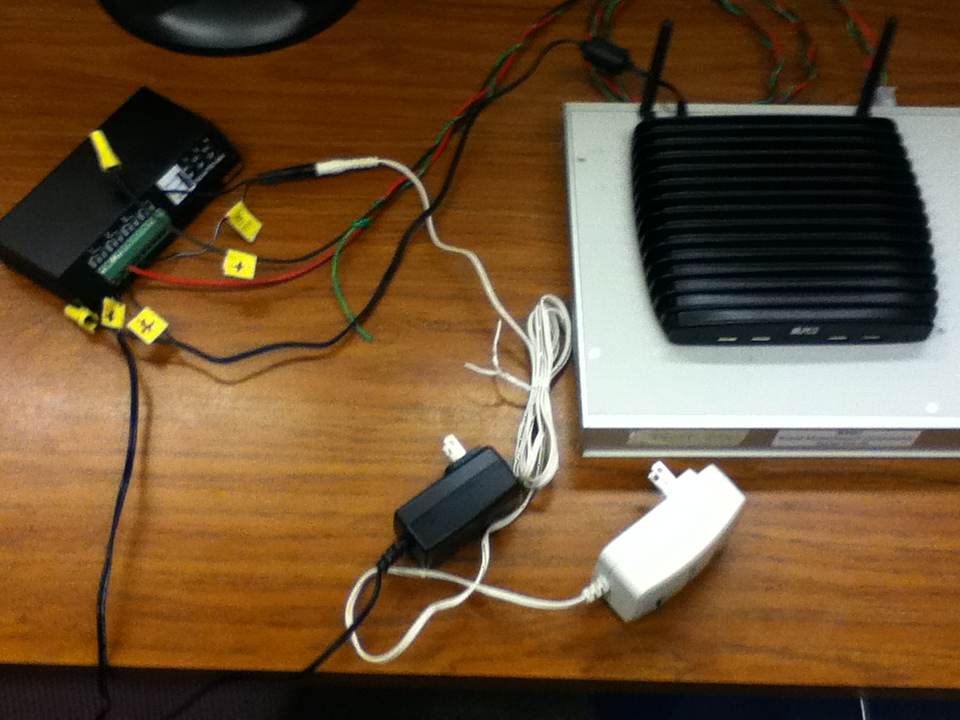
\includegraphics[scale=0.24]{pictures/power_rmg_computer.JPG}
  \end{center}
  \caption{Network powerswitch, field computer, and RMG receiver.}
  \vspace{-10pt}
\end{wrapfigure}
There are a number of products available that strike a comprimise between power consumption 
and processing power. The fit-PC3 suites our needs well.\footnote{For details, visit
\href{http://www.fit-pc.com}{\tt fit-pc.com}.} The fit-PC3 has a dual-core, 32-bit AMD
processor, 2 GBs of ram, and a 8GB solid state drive. Although it is designed to run 
any general-purpose desktop operating system, the fit-PC3 can easily be configured to 
run as a headless system. It even comes with a mini-rs232 console interface, although 
we don't make use of this in QRAAT. With our software running full-bore, the fit-PC3 
draws 46 W. 

\textbf{Powerswitch}. A network-addressible powerswitch makes it possible to turn the 
equipment on and off remotely and, with certain products, monitor power levels. We've 
deemed this feature necessary for two reasons: one, an intermittent issue related to 
the RMG receiver's USRP\footnote{For details, visit
\href{https://www.ettus.com}{\tt ettus.com}.} can be fixed by 
cycling the power; two, we need to be able to save energy. The powerswitch, field computer,
and network router are connected via an ethernet switch. The field computer and RMG 
receiver are powered by the powerswitch. The computer's power is switched over the 
network by the server, and the the computer is set up to switch the receiver. 

Again, there are various solutions for network power switching. Most of these input 
mains power, i.e. 120 V AC, and require us to mofidy them to work with our solar 
panels (12 V DC). The PingBrother EPIW104P\footnote{For details, visit
\href{http://www.pingbrother.com}{\tt pingbrother.com}.} passive POE ethernet switch 
not only allows us to input the proper power, but provides an array of features 
uesful for our deployment of QRAAT. The EPIW104P can switch a 12 V DC relay instead of
POE, and the ethernet ports can be used as a dumb switch. In addition, its http-based 
interface can be used to monitor the input voltage and power consumption. Our nominal 
hardware configuration with the PingBrother powerswitch and fit-PC3 is as follows: 

\begin{description}
  \item[\quad Network.] The network router and field computer are plugged into the 
    powerswitch's ethernet switch. The powerswitch and computer are assigned static
    IP addresses in the subnet of the router. Static addresses are necessary because 
    the QRAAT server must know how to reach the site; this information is not 
    distributed when the node comes into the network. (See software overview section 
    for details.) 
    
  \item[\quad Power.] The field computer's power is attached to the powerswitch's 
    first relay on NC ("normally closed"). If power goes down and is then made 
    availalbe, the field computer will be powered automatically. The RMG receiver is
    attached to the second relay on NO ("normally opened") so that it won't get power 
    automatically. 
    
\end{description}
 

\subsection{Software}

TODO 

\subsection{Usage}

TODO



\section{System specifications}
QRAAT has two main components: the remote field computers, which implement the initial 
signal detection, and the server, which collects data from the field computers for 
higher order processing. Here we outline the structure of these two components. 

\subsection{RMG Remote}
Each field computer is configured to run the software defined radio. We are using 
fanless, low-power machines manufactured by fit-PC.\footnote{For details, visit
\href{http://www.fit-pc.com}{\tt fit-pc.com}.} The fit-PC3 has a dual-core, 32-bit AMD
processor, 2 GBs of ram, and 8 GBs solid-state persistent memory. They 
run stock Ubuntu Server 12.04. Along with the SDR implemented in GNU Radio, each is 
configured to run an ssh server, ntpdate, and other necessities. 

The initial signal processing software outputs files corresponding to pulses 
with the extension \texttt{.det}. These are stored on a temporary file system in memory, 
located at /tmp/ramdisk/det\_files. The pulse data files are stored in a directory 
structure according to the the minute in which they were recorded, for example: 
\begin{verbatim}
  /tmp/ramdisk/det_files/2013/03/22/15/20/03439743.det
\end{verbatim}
The file name gives the second it was created with millisecond precision, i.e. 
\texttt{SSUUUUUU.det}. This is the last step on the field computers; these files are 
then collected by the server. 

Each site has a user called \textit{rmg} whose password---you guessed it---is \textit{rmg}. 

The QRAAT software is located in /home/rmg/QRAAT. We've set it up as a git 
repository that pulls from the RMG Server. To update the software, ssh to the site, 
switch to this directory, and type '\texttt{git pull}'. You will be prompted for 
the server's password.  

The transmitter file is /home/rmg/tx.csv. 

\subsection{RMG Server}
Along with managing the field computers and collecting data, the server is responsible for
callibration and triangulation. The \texttt{rmg} script allows us to power the computer and 
RMG module on and off, cycle the RMG module power, start and stop the software defined radio, 
update the field computer's transmitter file, and collect \texttt{.det}s. The server has a 
file called \texttt{sitelist.csv} that stores various parameters and the status of the RMG remotes:
\begin{enumerate}
  \item \textit{Name} - of the site, 
  \item \textit{CompIP} - hostname or IP address of the remote computer, 
  \item \textit{PowerIP} - hostname or IP address of the network addressible power source,
  \item \textit{CompOutlet} - outlet number of the computer, 
  \item \textit{RxOutlet} - outlet number of the RMG receiver module, 
  \item \textit{PowerType} - power source type, e.g. Netbooter, PingBrother, or WebPowerSwitch, and finally
  \item \textit{State} - is the site up, down, or active (SDR is running). 
\end{enumerate}
Following is a sample of a typical \texttt{sitelist.csv} file. Fields can be skipped if they aren't applicable
to a particular site (e.g. site1 runs on the same machine as the server), but they must be deliniated by 
commas:
\begin{verbatim}
name,comp_ip,power_ip,comp_outlet,rx_outlet,powertype,state
site0,10.0.0.55,10.0.0.56,1,2,pingbrother,active
site1,localhost,,,,,active
site2,10.2.1.55,10.2.1.56,1,2,netbooter,down
site10,10.10.1.55,10.10.1.56,1,2,webpowerswitch,up
\end{verbatim}

\texttt{rmg} uses RSA encryption for ssh instead of prompting the user for a password each time. This is 
important since some of \texttt{rmg}'s routines, such as \texttt{rmg fetch}, make many ssh calls. The 
RMG remotes store the public part of the key and the server the private part. 

We keep a copy of the software repository on the server from which the remote ocmputers pull; the server 
copy pulls directly from github. 




\section{Configuration instructions}

\subsection{Field computers}
The field computers were configured by building and installing the software on one 
system, creating an image from its harddrive, and copying this image to the other sites. To create
the image, we first installed a stock copy of Ubuntu Server 12.04 on a 7.5 GB partition, leaving
512 MB for swap. We configured no automatic updates, since these computers spend the majority of 
their time not connected to the internet. After booting the system and updating, the first thing
to do is install the following packages via apt-get: 
\begin{enumerate}
  \item \texttt{git-core} - clone our software repository from github,
  \item \texttt{openssh-server} - each field site needs to run an ssh daemon,
  \item \texttt{minicom} - serial interface to RMG receiver module, and
  \item \texttt{ntpdate} - remote computers will be clock synced to the server via \texttt{ntpd}. 
\end{enumerate}

\subsubsection{Building and installing the software}
Clone the online repository to get things going:
\begin{verbatim}
$ git clone github.com/QRAAT/QRAAT.git
\end{verbatim}
The first thing to build is GNU Radio along with the UHD driver. For conveniance, we provide a copy 
of the gnuradio build script written by Marcus Leech. Type
\begin{verbatim}
$ QRAAT/build-gnuradio -v all
\end{verbatim}
to start downloading and building. This may take a few hours; however, you'll only need to do this once. When the 
build finishes, it will output a couple post-install tasks. Make sure you do these. Next, building
and installing the QRAAT software is essentially the same procedure, though it will take less than 
two minutes: 
\begin{verbatim}
$ QRAAT/build-rmg -v install
\end{verbatim}

Before testing your build, we need to setup communication with the RMG recevier's PIC interface. First we 
add a rule to udev\footnote{\texttt{udev} is a common domain on GNU/linux systems used to handle 
new devices when they're plugged in. For instance, when you installed GNU Radio, rules were installed 
for the USRP---a hardware component of the RMG receiver---and the UHD driver.} to set permissions for 
\texttt{/dev/ttyUSB0}, the serial interface for the RMG receiver. Create a new file: 
\begin{verbatim}
$ sudo vi /etc/udev/rules.d/101-serial-usb.rules
\end{verbatim}
and type the following line: 
\begin{verbatim}
  KERNEL=="ttyUSB0", MODE="0666"
\end{verbatim}
To verify that this worked, we'll try to communicate with the PIC via minicom. Open up the minicom
configuration screen. Under \textit{Serial port setup}, set \textit{Serial Device} to \texttt{/dev/ttyUSB0}.
Set \textit{Bps/Par/Bits} to \texttt{9600 8N1}. Lastly, set \textit{Hardware/Software Flow Control} to 
\texttt{No}. Restart minicom. See if you're able to communicate with it by typing "\texttt{?}".  

\subsubsection{Post-configuration} 

We don't want the RMG remotes to save their pulse data locally to disk; the files will be stored
locally in memory. For this reason, we need to set up a ramdisk to be created at start up. Add 
the following line to the end of \texttt{/etc/fstab} (be careful!): 
\begin{verbatim}
tmpfs   /tmp/ramdisk  tmpfs  nodev,nosuid,mode=1777,size=1024M   0   0
\end{verbatim}
1 GB is reasonable since the field computers have 2 GBs of ram. 

If linux shutsdown uncleanly, e.g. the site loses power, the GRUB bootloader will wait for user 
input before rebooting the operating system. This is bad for headless systems, so we need to 
configure GRUB to timeout in this situation. Add the following to /etc/default/grub: 
\begin{verbatim}
  GRUB_RECORDFAIL_TIMEOUT=2
\end{verbatim}
Then type \texttt{sudo update-grub}. 

Up until now, we've been using the field computer with a monitor, keyboard, and ethernet connection
to the internet. The next thing we have to do is configure the network interface so that we can 
access it over ssh without a head. In /etc/network/interfaces, comment out the default 
ethernet interface and add a static IP address: 
\begin{verbatim}
  # auto eth0
  # iface eth0 inet dhcp
  auto eth0
  iface eth0 inet static
    address 10.20.1.55
    netmask 255.0.0.0
\end{verbatim}
To connect to the computer directly through an ethernet cable, just setup a static IP address on 
the host system in the same subnet. See the section on networking for details. 

The next thing to do is change the system's hostname. This needs to be changed in two places:
/etc/hostname and /etc/hosts. 

Lastly, since we will be managing the power of this system remotely, we want to be able to 
shutdown and reboot the computer without typing in a sudo password. Type 
\begin{verbatim}
$ sudo visudo
\end{verbatim}
and add the following lines to the end of the sudoers file: 
\begin{verbatim}
  rmg ALL=NOPASSWD: /sbin/halt
  rmg ALL=NOPASSWD: /sbin/reboot
  rmg ALL=NOPASSWD: /sbin/poweroff
\end{verbatim}

\subsubsection{Creating an image}
The preceeding configuration is time-consuming, though not difficult. For configuring many sites, 
it's best to create an image from a fully configured system and copy this to other sites. The 
simplest way to do this is with a Ubuntu live-USB. Plug a monitor, keyboard, and mouse into the 
FitPC and boot a live copy of Ubuntu on a thumbdrive. Grab a terminal and make sure the harddrive
is unmounted. ("\texttt{mount | grep "sda"}. Verify that /dev/sda is indeed the 
harddrive.) Plug in an external harddrive or thumbdrive that can 
fit the 8 GB file we're about to create. Change the directory to the external drive and run: 
\begin{verbatim}
$ dd if=/dev/sda of=qraat.img bs=4K 
\end{verbatim}
To copy the image, boot another computer in the same way. Plug in the external drive, change to 
its directory, and type
\begin{verbatim}
$ dd if=qraat.img of=/dev/sda bs=4K
\end{verbatim}

Both of these commands should take about 30 minutes. Once you've finished copying the image, you'll 
want to edit the hostname and network interfaces as described in the preceeding section.  



\subsection{Networking}
Here are the configuration steps that need to be taken as of this writing (27 March).

\subsubsection{West campus prototype}
We won't have networking for this implementation. As they are the ethernet interfaces of the RMG 
remotes are configured with a static IP address 10.\texttt{<site\_no>}.1.55 and netmask 255.0.0.0. 
To connect to it, the simplest thing to do is create an interface 
in network manager. \textit{Network Manager} $\rightarrow$ \textit{Edit Connections...}, in the 
\textit{Wired} tab, choose \textit{Add}. In \textit{IPv4 Settings}, choose \textit{Method = Manual}. 
Add an address like 10.253.1.55 with netmask 255.0.0.0. You should be good to go.  

In lue of networking, we're collecting the data on external harddrives at all three sites. We 
can use udev to setup automounting, Create a new udev rule file, like /etc/udev/rules.d/
90-hd-backup.rules and add the following lines:
\begin{verbatim}
ACTION=="add", SUBSYSTEMS=="scsi", KERNEL=="sd[a-h]1", RUN+="/bin/mount /dev/%k /media/backup"
ACTION=="remove", SUBSYSTEMS=="scsi", KERNEL=="sd[b-h]1",RUN+="/bin/umount /dev/%k"
\end{verbatim}


\subsubsection{Quail Ridge}
The ethernet interface needs to be configured to use the Qurinet router as its gateway. 
In /etc/network/interfaces, you'll find an interface that is commented out. 
Uncomment this and comment out the old one. 
\begin{verbatim}
  # Default interface in Quirinet
  auto eth0 
  iface eth0 inet static
    address 10.20.1.55
    netmask 255.255.0.0
    gateway 10.20.1.1
\end{verbatim}

The second part is to make sure the git repository is pointed to the right place. In 
/home/rmg/QRAAT/.git/config, you'll find a line that reads
\begin{verbatim}
  url = christopher@10.253.1.55:work/QRAAT # change me!
\end{verbatim}
Change this to the correct user and directory and you're set!

\end{document}
